% !TeX root = ../../thesis.tex

\subsection{The need for Agile}
In the wake of the world economic crisis, software companies were forced to devote efforts into researching how their overall expenses could be reduced. This research has concluded that in order to reduce financial risks, the \emph{time-to-market} of an application should be as short as possible. In order to accomplish this, further research was conducted, resulting in an increase of attention for agile methodologies in scientific literature \cite{ionel2009}. As was previously described in \autoref{sssec:agilevalue-workingsoftware}, agile methodologies strive to deliver a minimal version as soon as possible, allowing additional functionality to be added in an incremental fashion. This effectively results in a shorter \emph{time-to-market} and lower costs, since the company can decide to cancel the project much earlier in the process.\\

\noindent In addition to a reduced time-to-market, maintaining an agile workflow has also proven beneficial to the success rate of development. A study performed by The Standish Group revealed that the success rate of agile projects is more than three times higher compared to when traditional methodologies are practised, as illustrated in \autoref{fig:agile-success-rate}. 

\begin{figure}[htbp!]
	\centering
	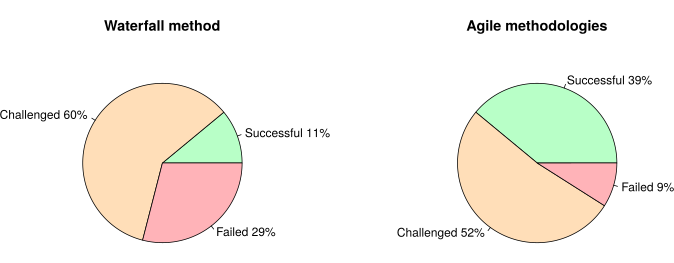
\includegraphics[width=\textwidth]{assets/charts/agile-success-rate.pdf}
	\caption{Success rate of Agile methodologies \cite{standish2015chaos}.}
	\label{fig:agile-success-rate}
\end{figure}